%%MAIN: thesis.tex

%%%%% The Validation %%%%%
\chapter{Implementation: Lesson Plans} \label{ch_teaching}

In its current form, the ``Processing Abstractions'' environment as presented in chapter \ref{ch_pa} is mainly targetted at the obligatory introduction to computer sciences at high school level.

Before going into empirical results from using this environment in two courses, three lesson plans will be presented for which it has been developed: a \emph{Sichtenwechsel} in computer architecture (section \ref{sc_lesson_ca}); an introduction into the inner workings of a compiler (section \ref{sc_lesson_compiler}); and first a plan for a general introduction to programming (section \ref{sc_lesson_intro}). Some ideas for how to expand it for other school levels will be presented in section \ref{sc_lesson_other}.

For all the lessons, students will need a local environment of ``Processing Abstractions'' installed on a computer available to them. See appendix \ref{app_setup} for how to set it up. Additionally, for non-German speaking students the contents will have to be translated to the teaching language.



\section{Introduction to Programming} \label{sc_lesson_intro}

While the ``Processing Abstractions'' environment has been developed for linking programming and computer architecture, it can also be used for an introduction to programming. This does even help linking programming and computer architecture for students, since they can start at the same point and reuse the experience already gained.


\subsection{Educational objective}

After the introduction, students should \dots
\begin{itemize}
\item be able to work within GT.
\item be able to read, write and understand programs with a limited command set, including working with the implicit animation loop.
\item be able to learn from their mistakes, correct themselves and not be afraid of breaking things.
\end{itemize}

In the end, students should have a solid foundation for taking on the task of writing a basic but still interesting app or game.\footnote{Possible ideas, which all have been implemented by students, include: ``Flappy Bird'', ``Geometry Dash'', ``Pong'', ``Doodle Jump'', ``Snake'', a quiz, a labyrinth, \emph{etc.}. For most of these, ``Processing Abstractions'' provides sufficent support, the main deficit being the lack of keyboard input.}


\subsection{Prerequisites}

Students need experience in using their own computer, including \dots
\begin{itemize}
\item downloading and extracting archives, and
\item dealing with their virus scanner.\footnote{At least under Windows, many scanners flag GT as untrustworthy due to its executable lacking a valid signature. Some virus scanners even block the entire download, if the archive is distributed over a network.}
\end{itemize}

Additionally, the teacher must prepare their contents in GT e.\,g. as described in \ref{app_setup} and distribute them. Ensure that the first lesson page will be displayed on first startup.


\subsection{Introduction to Glamorous Toolkit} \label{ssc_lesson_gt}

Since Glamorous Toolkit will be a new environment altogether for all students, some basics on its usage have to be introduced first within ten minutes:

\begin{instructions}
\item Ask students to download and extract your GT distribution as homework for the first lesson. Under Windows, they might run into a first issue with their virus scanner blocking the download, so remind them about what to do in that case.\footnote{In most virus scanner settings, the warning can be overruled by the user; else they might have to \emph{temporarily} disable scanning for this one download.}
\item Tell students to start GT and open the notebook page about working with Glamorous Toolkit (``Arbeiten mit Glamorous Toolkit'' in the included teaching materials). Also ask them to help their neighbours, if they see them struggling. Use the time while students are reading and doing the first tasks for ensuring that everyone has managed to get GT running.
\item Introduce GT as an interactive notebook similar to what students already know from class.\footnote{Many schools have standardized on working with the Microsoft 365 Office Suite which includes OneNote.} One main difference will be that additional views will open to the side, hiding the table of contents. So show them, how to get back by selecting the left-most view (through the blue dots at the center top) and expand it (through the $+$ at the top left).
\item If you want students to be able to take notes of their own inside GT notebooks, show them how to move a page to their local knowledge base (where it can be backed up individually) and how to create and structure new paragraphs (\ct{Ctrl+Enter}, \ct{Alt+Shift+Arrow}). Markdown syntax for formatting does not have to be introduced explicitly, that can be replicated by students by inspecting your content.
\item Finally, keep in mind GT's ability to be inspected at every level and point more advanced students towards using these (e.\,g. by \ct{Ctrl+Shift+Alt+Click} anywhere, by double-clicking on list items, or by going through the different views of an object).
\end{instructions}

Please note that as described in \ref{sc_gt}, GT is bleeding edge technology and might not always behave the way you and your students have become used to: Since notebook pages are rendered progressively, scrolling won't always work smoothly (and will scroll inner content, if the mouse cursor isn't positioned at a page's border); occasionally unexpected error messages trigger the debugger to pop up which has to be closed again; and sometimes the keyboard modifiers may get stuck, resulting in shortcuts no longer working (which is resolved by switching to a different app and back).


\subsection{Lesson Plans}

Since this isn't the focus of this thesis, we won't go into much detail about introducing programming, but just summarize what might work within the provided environment:

Start top down as suggested in \ref{ssc_top_down} from either abstract art or games\footnote{Most one-tap games should work, e.\,g. \url{https://www.lessmilk.com/almost-pong/} has reasonably simple gameplay with minimalist visuals.} and start dissecting how this concrete entity might be described, first in natural language and then in formalized language.

Then follow Reas and Fry \cite{Rea14} and introduce the Processing language (see \ref{sc_processing}), by starting with a sequence of statements with few commands (e.\,g. \ct{size}, \ct{rect}, \ct{ellipse} and \ct{fill}), and then sequentially introducing comments, colors, variables and arithmetic, the animation loop, conditions and interactivity.

Every concept can be described on a notebook page with given examples for first exploring the effects of a command and its arguments\footnote{Students may either describe the expected behavior and then verify that their expectation matches the outcome, or less taxingly try given or random values and then describe their observations. Variations consist e.\,g. in a student describing desired behavior and then (another student) trying to achieve this.} and then later using the concept for solving problems by starting from a skeleton program (see figure \ref{fig_screenshot_introduction} for an example of both).

\begin{cfigure}[fig_screenshot_introduction]{Excerpt from an interactive notebook page with exploratory and live programming tasks.}
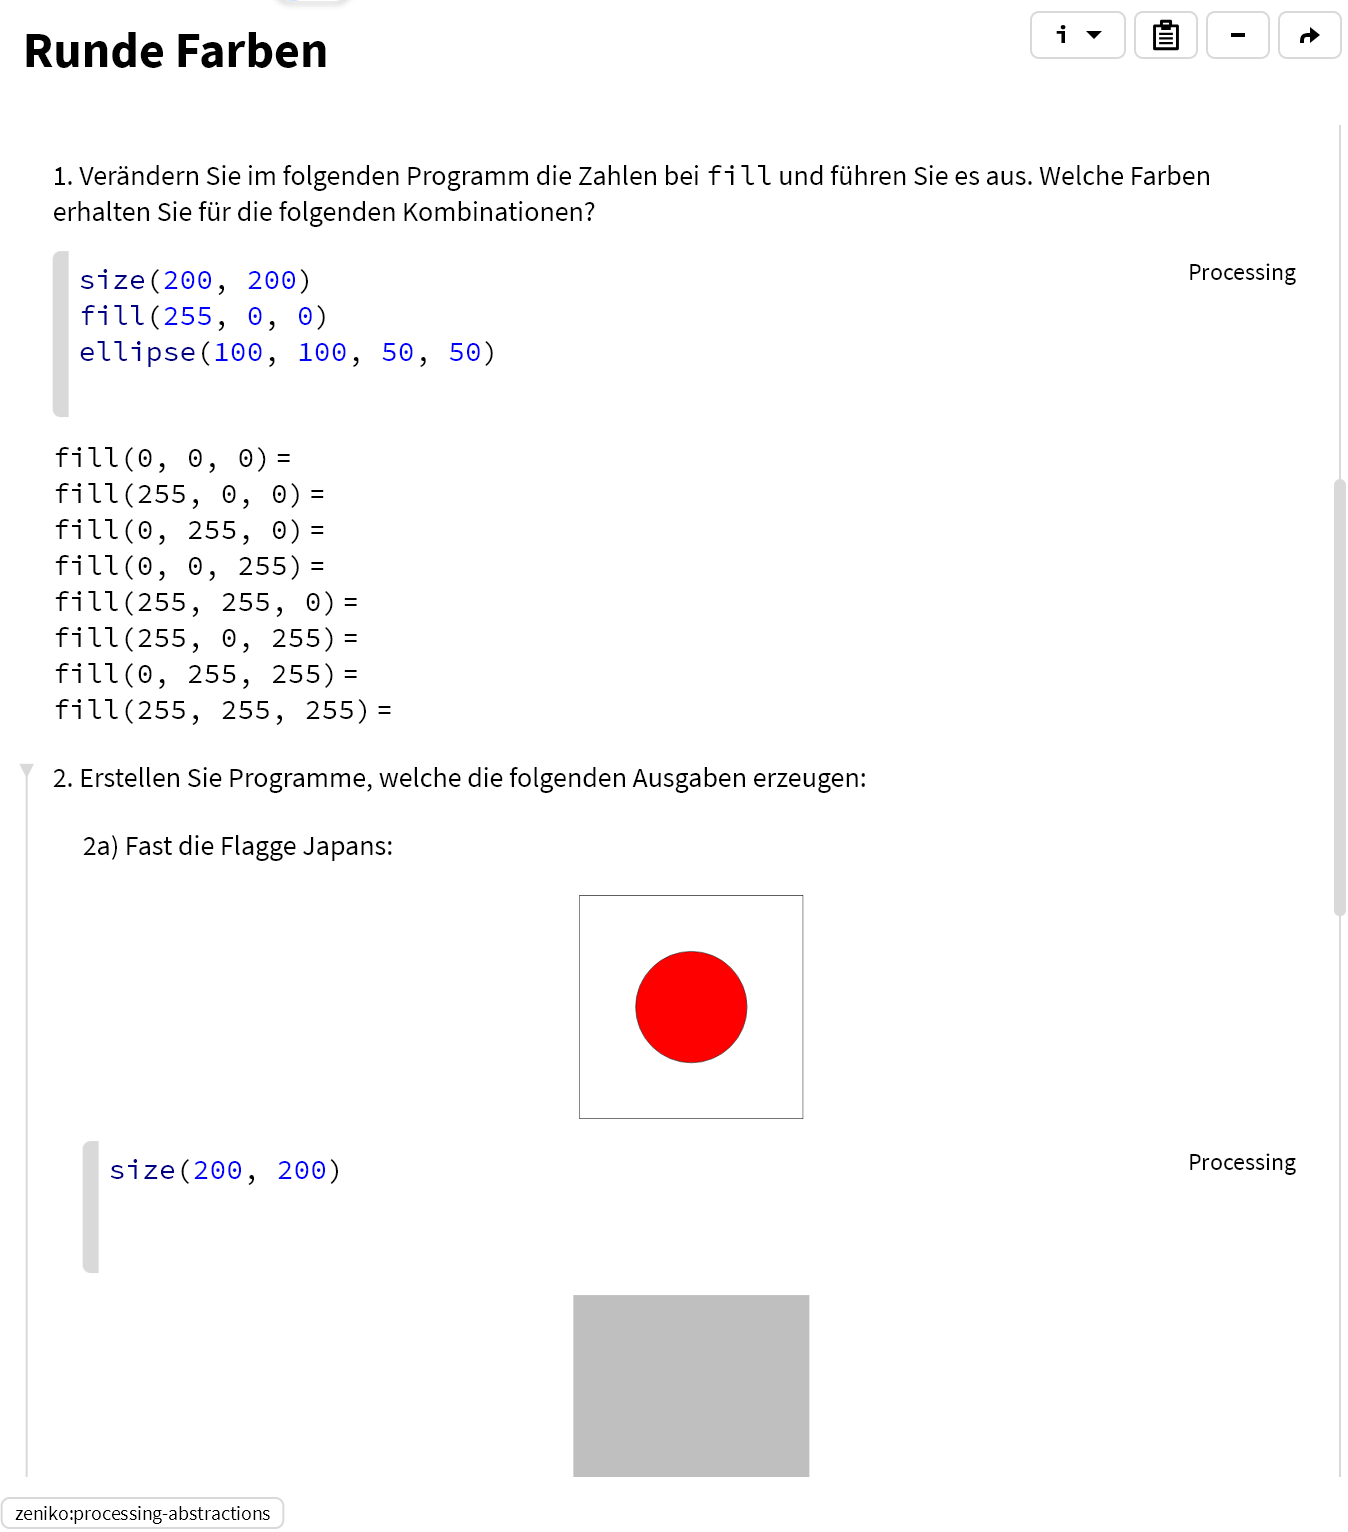
\includegraphics[width=.7\textwidth]{screenshot_introduction}
\end{cfigure}

At the beginning, debugging will only consist in modifying values and observing live changes until the desired output is reached. At later stages, the step-by-step execution views will be useful, where executed expression, variable values and visual output are displayed side-by-side and execution can be played forward and also in reverse.

Quicker and more proficient students could also already at this point start to delve deeper: The third and fourth execution icons will lead them to discover by themselves what lies under the hood.

Sample content for this is included in the \emph{Unterrichtsmaterialien} of  ``Processing Abstractions'' as ``\emph{Programmieren mit Processing}''.



\section{Lesson on Computer Architecture} \label{sc_lesson_ca}

The main objective of this thesis was to demonstrate, how understanding of what happens when executing a program could be improved by having students perform a \emph{Sichtenwechsel}. The same goes for the other way around, where computer architecture is explained in more concrete form by tying it to previous programming experience.

Introductions to computer science which extend beyond a pure programming course often contain lessons on computer architecture. E.\,g. the curriculum \cite[p.\,145]{Erz16} asks for students to ``know how computers and networks are structured and work''.

We again propose to approach this task top down (see \ref{ssc_top_down}) and move along the path specified in figure \ref{fig_multitier}. This will be outlined here with validation of part of this approach following in \ref{sc_validation_ca}.

With respect to manageability (see \ref{ssc_manageability}), it is proposed to mostly skip the inner workings of a compiler and treat that in a separate sequence (maybe only for students specializing in computer science).


\subsection{Educational objective}

After these lessons, students should \dots
\begin{itemize}
\item be able to explain the concepts of (virtual) machine, memory, stack, machine language, and program counter (with relation to a von Neumann model).
\item have a notion of why machine language must be different from a high-level language such as Processing.
\item be able to explain why some commands are slower than others.
\item connect their knowledge about encodings with how values and machine code are stored.
\item consequently understand how one of their programs might be run on actual hardware and document their understanding with correct terms.
\end{itemize}


\subsection{Prerequisites}

Students must already have basic programming skills in a high level language. In particular, they must know about variables and loops. If they don't know Processing or at least Python yet, a brief introduction (maybe along the ideas proposed in \ref{sc_lesson_intro} above) is required.


\subsection{Lesson Plan}

Whereas Nisan and Schocken \cite{Nis21} introduce their bottom up course with a top down overview, we propose doing the same in reverse for this top down approach:

\begin{instructions}
\item Start with a brief repetition on programming by giving students a few quickly solved tasks (including one about the animation loop, where at least the skeleton structure is given). If this is the student's first encounter with Glamorous Toolkit, use this opportunity to introduce it (see \ref{ssc_lesson_gt}).
\item Show students the innards of a computer and ask where their programs reside in there. Use this for discussing hard drives and volatile memory, and a repetition about encodings and how everything boils down to \texttt{1}s and \texttt{0}s (or current and no current respectively).
\item Briefly start at the desired lowest abstraction layer, e.\,g. (light) switches, and explain how they're used for creating processors.
\item 



\item Finally, treat circuits, logic gates, transistors and maybe down to silicon outside of GT to the desired depth.
\end{instructions}

The more students are supposed to work on their own, the more they'll need an overview over the different layers prior to combining them. As a prerequisite, it is recommended to at least introduce the Von Neumann architecture and its split of the CPU into control unit and arithmetic unit (see figure \ref{fig_von_neumann}).

\begin{cfigure}[fig_von_neumann]{Von Neumann architecture.}
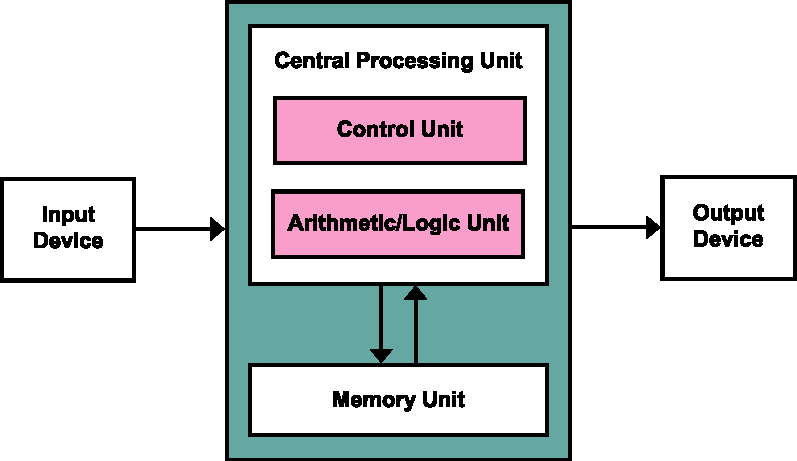
\includegraphics[width=10cm]{Von_Neumann_Architecture}
\begin{todo}
\item replace or properly attribute: Kapooht, 2013, CC BY-SA 3.0
\end{todo}
\end{cfigure}


\begin{cfigure}[fig_screenshot_vm_execution]{Excerpt from an interactive notebook page on .}
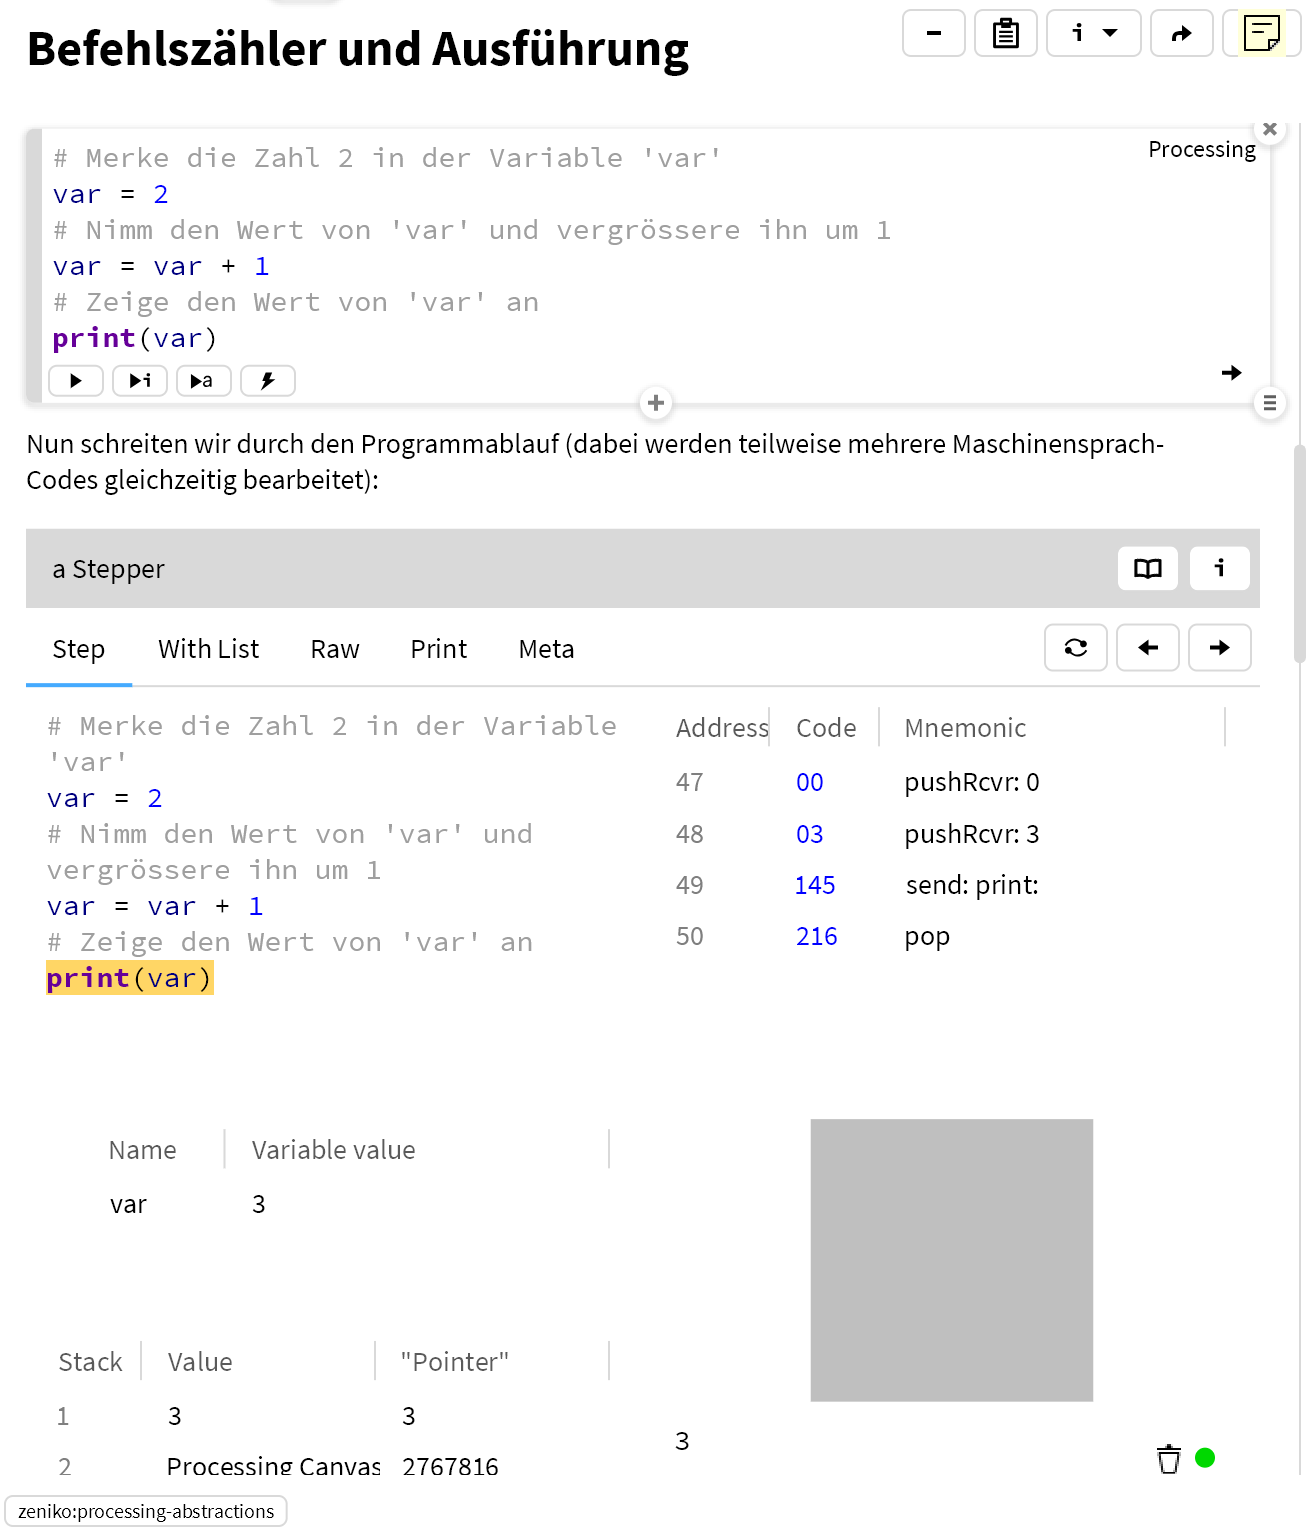
\includegraphics[width=.7\textwidth]{screenshot_vm_execution}
\begin{todo}
\item Decide which screenshots belong into the appendix instead.
\end{todo}
\end{cfigure}



\section{Lesson on Compilers} \label{sc_lesson_compiler}

Using PA to demonstrated the steps of lexing, parsing, transpiling, compiling and optimizing.

Part of this has been validated (cf. \ref{sc_validation_compiler})


\subsection{Educational objective}

\begin{todo}
\item students can explain the difference between high and low level language
\item students can enumerate the steps required for compiling a program
\item students have an understanding of the roles a lexer, parser, transpiler and compiler play
\end{todo}


\subsection{Prerequisites}

\begin{todo}
\item programming with Processing (e.\,g. from \ref{sc_lesson_intro})
\item GT/PA installed (e.\,g. from \ref{ssc_lesson_gt})
\item Stacks and registers
\end{todo}


\subsection{Lesson Plan}

\begin{todo}
\item Repetition high level programming (see tasks in PA)
\item Comparision with low level programming (e.\,g. \cite{Tom15}): levels 1 to 6 (introduces jumps, memory access, arithmetic)
\item Presenting/reading overview, compare with natural language
\item Lexer: compare given example with mainly different whitespace; what are tokens?
\item Parser: describe AST in own words, compare with sentence structure from natural languages; develop simple parsing model (better views?)
\item Transpiler (optional): compare Processing and Smalltalk
\item Compiler: compare AST with intermediary representation; compare Program with intermediary representation; compare intermediary representation with \cite{Tom15}
\item Optimization: naive examples
\end{todo}



\section{Further Lesson Ideas} \label{sc_lesson_other}

Connecting PA with Smalltalk; extend it to object oriented programming; mould the environment to questions developed during the course; \dots
